% !TEX root = learner4_block_diagram.tex
% Comprehensive block diagram for Learner 4 (L1--L6).
% Compile from this directory:
%   pdflatex -output-directory=../outputs/learner4 learner4_block_diagram.tex
% Or:  ./scripts/build_learner4_block_diagram.sh

\documentclass[11pt]{article}
\usepackage[landscape,margin=0.35in]{geometry}
\usepackage{amsmath,amssymb}
\usepackage{tikz}
\usetikzlibrary{positioning,arrows.meta,calc,fit,shapes.geometric,backgrounds,decorations.pathreplacing}
\usepackage{xcolor}

\definecolor{handc}{RGB}{180,95,30}      % hand / action
\definecolor{plantc}{RGB}{140,30,40}     % true plant
\definecolor{ekfc}{RGB}{27,54,93}        % EKF / belief
\definecolor{schedc}{RGB}{30,107,58}     % schedule / xi
\definecolor{failc}{RGB}{130,50,140}     % failure gate
\definecolor{scorec}{RGB}{70,70,70}      % scoreboards
\definecolor{boxfill}{RGB}{248,248,250}
\definecolor{eqfill}{RGB}{252,252,248}
\definecolor{arrowgrey}{RGB}{70,70,70}

\begin{document}
\thispagestyle{empty}
\begin{center}
{\Large\bfseries Learner~4 --- one-trial block diagram}\\[0.15em]
{\small Co-contract to learn? \quad
\texttt{order\_reduction/experiment4.py} \texttt{run\_seed} \quad
plant $G^\star$ fixed; only $\xi$ and model capacity vary}\\[0.35em]
\end{center}

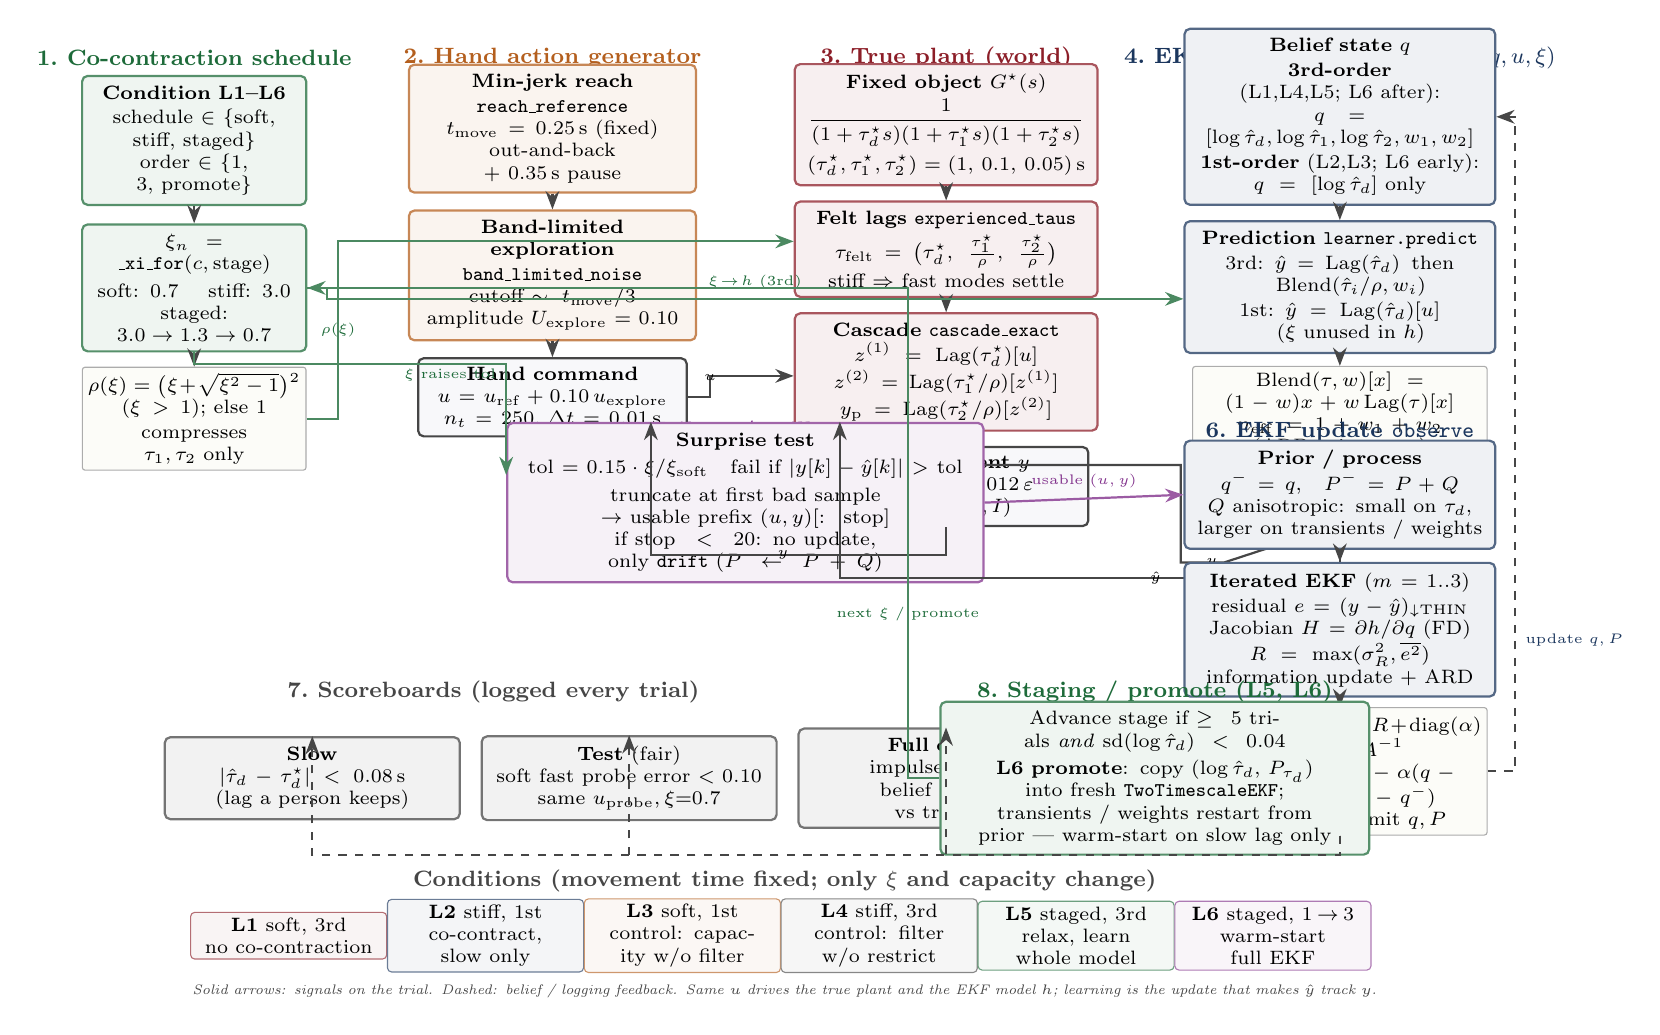
\begin{tikzpicture}[
  >=Stealth,
  font=\scriptsize,
  node distance=0.28cm and 0.32cm,
  blk/.style 2 args={
    rectangle, rounded corners=2pt, draw=#1!75, fill=#1!7,
    thick, align=center, inner sep=3.5pt, text width=#2
  },
  tinyblk/.style 2 args={
    rectangle, rounded corners=1.5pt, draw=#1!65, fill=#1!5,
    thin, align=center, inner sep=2pt, text width=#2
  },
  io/.style={
    rectangle, rounded corners=2pt, draw=arrowgrey, fill=boxfill,
    thick, align=center, inner sep=3pt, text width=#1
  },
  eq/.style={
    rectangle, rounded corners=1pt, draw=arrowgrey!45, fill=eqfill,
    thin, align=center, inner sep=2pt, font=\scriptsize
  },
  arr/.style={->, thick, draw=arrowgrey},
  darr/.style={->, thick, draw=arrowgrey, dashed},
  farr/.style={->, thick, draw=#1!80},
  title/.style={font=\bfseries\footnotesize, text=#1},
]

% =====================================================================
% COLUMN A --- schedule / grip
% =====================================================================
\node[title=schedc] (schedtitle) at (0, 8.6) {1.\ Co-contraction schedule};
\node[blk={schedc}{2.6cm}] (cond) at (0, 7.55)
  {\textbf{Condition L1--L6}\\[1pt]
   schedule $\in$ \{soft, stiff, staged\}\\
   order $\in$ \{1, 3, promote\}};
\node[blk={schedc}{2.6cm}, below=0.22cm of cond] (xibox)
  {$\xi_n = \texttt{\_xi\_for}(c,\mathrm{stage})$\\[2pt]
   soft: $0.7$ \quad stiff: $3.0$\\
   staged: $3.0\!\to\!1.3\!\to\!0.7$};
\node[eq, below=0.18cm of xibox, text width=2.7cm] (rhoeq)
  {$\rho(\xi)=\bigl(\xi+\sqrt{\xi^2-1}\bigr)^2$\\
   $(\xi>1)$; else $1$\\[1pt]
   compresses $\tau_1,\tau_2$ only};

\draw[arr] (cond) -- (xibox);
\draw[arr] (xibox) -- (rhoeq);

% =====================================================================
% COLUMN B --- hand action generator
% =====================================================================
\node[title=handc] (handtitle) at (4.55, 8.6) {2.\ Hand action generator};
\node[blk={handc}{3.4cm}] (minjerk) at (4.55, 7.7)
  {\textbf{Min-jerk reach}\\[1pt]
   \texttt{reach\_reference}\\
   $t_{\mathrm{move}}=0.25$\,s (fixed)\\
   out-and-back + 0.35\,s pause};
\node[blk={handc}{3.4cm}, below=0.2cm of minjerk] (explore)
  {\textbf{Band-limited exploration}\\[1pt]
   \texttt{band\_limited\_noise}\\
   cutoff $\sim t_{\mathrm{move}}/3$\\
   amplitude $U_{\mathrm{explore}}=0.10$};
\node[io=3.2cm, below=0.2cm of explore] (u)
  {\textbf{Hand command}\\
   $u = u_{\mathrm{ref}} + 0.10\,u_{\mathrm{explore}}$\\
   $n_t=250$, $\Delta t=0.01$\,s};

\draw[arr] (minjerk) -- (explore);
\draw[arr] (explore) -- (u);

% =====================================================================
% COLUMN C --- true plant
% =====================================================================
\node[title=plantc] (planttitle) at (9.55, 8.6) {3.\ True plant (world)};
\node[blk={plantc}{3.6cm}] (object) at (9.55, 7.75)
  {\textbf{Fixed object} $G^\star(s)$\\[1pt]
   $\displaystyle\frac{1}{(1+\tau_d^\star s)(1+\tau_1^\star s)(1+\tau_2^\star s)}$\\[2pt]
   $(\tau_d^\star,\tau_1^\star,\tau_2^\star)=(1,\,0.1,\,0.05)$\,s};
\node[blk={plantc}{3.6cm}, below=0.18cm of object] (felt)
  {\textbf{Felt lags} \texttt{experienced\_taus}\\[1pt]
   $\tau_{\mathrm{felt}}=\bigl(\tau_d^\star,\;
     \tfrac{\tau_1^\star}{\rho},\;\tfrac{\tau_2^\star}{\rho}\bigr)$\\[1pt]
   stiff $\Rightarrow$ fast modes settle};
\node[blk={plantc}{3.6cm}, below=0.18cm of felt] (cascade)
  {\textbf{Cascade} \texttt{cascade\_exact}\\[1pt]
   $z^{(1)}=\mathrm{Lag}(\tau_d^\star)[u]$\\
   $z^{(2)}=\mathrm{Lag}(\tau_1^\star/\rho)[z^{(1)}]$\\
   $y_{\mathrm{p}}=\mathrm{Lag}(\tau_2^\star/\rho)[z^{(2)}]$};
\node[io=3.4cm, below=0.18cm of cascade] (y)
  {\textbf{Measurement} $y$\\
   $y = y_{\mathrm{p}} + 0.012\,\varepsilon$\\
   $\varepsilon\sim\mathcal N(0,I)$};

\draw[arr] (object) -- (felt);
\draw[arr] (felt) -- (cascade);
\draw[arr] (cascade) -- (y);
\draw[farr=schedc] (rhoeq.east) -- ++(0.4,0) |- ($(felt.west)+(0,0.1)$)
  node[pos=0.2, above, font=\tiny, text=schedc] {$\rho(\xi)$};
\draw[arr] (u.east) -- ++(0.28,0) |- ($(cascade.west)+(0,-0.05)$)
  node[pos=0.15, above, font=\tiny] {$u$};

% =====================================================================
% COLUMN D --- EKF measurement / plant model (belief)
% =====================================================================
\node[title=ekfc] (ekftitle) at (14.55, 8.6) {4.\ EKF measurement model $h(q,u,\xi)$};
\node[blk={ekfc}{3.7cm}] (state) at (14.55, 7.85)
  {\textbf{Belief state} $q$\\[1pt]
   \textbf{3rd-order} (L1,L4,L5; L6 after):\\
   $q=[\log\hat\tau_d,\log\hat\tau_1,\log\hat\tau_2,w_1,w_2]$\\[1pt]
   \textbf{1st-order} (L2,L3; L6 early):\\
   $q=[\log\hat\tau_d]$ only};
\node[blk={ekfc}{3.7cm}, below=0.18cm of state] (hmodel)
  {\textbf{Prediction} \texttt{learner.predict}\\[1pt]
   3rd: $\hat y=\mathrm{Lag}(\hat\tau_d)\,$ then\\
   \quad$\mathrm{Blend}(\hat\tau_i/\rho,w_i)$\\[1pt]
   1st: $\hat y=\mathrm{Lag}(\hat\tau_d)[u]$\\
   \quad($\xi$ unused in $h$)};
\node[eq, below=0.15cm of hmodel, text width=3.6cm] (blend)
  {$\mathrm{Blend}(\tau,w)[x]=(1-w)x+w\,\mathrm{Lag}(\tau)[x]$\\
   $n_{\mathrm{eff}}=1+w_1+w_2$ \ (ARD prior on $w$)};
\node[io=3.5cm, below=0.15cm of blend] (yhat)
  {\textbf{Predicted feel} $\hat y=h(q,u,\xi)$};

\draw[arr] (state) -- (hmodel);
\draw[arr] (hmodel) -- (blend);
\draw[arr] (blend) -- (yhat);
\draw[farr=schedc] (xibox.east) -- ++(0.25,0) |- ($(hmodel.west)+(0,-0.15)$)
  node[pos=0.75, above, font=\tiny, text=schedc] {$\xi\!\to\!h$ (3rd)};
\draw[arr] (u.south) -- ++(0,-0.35) -| ($(yhat.south west)+(-0.15,-0.35)$)
  -- ++(0.55,0) -- ($(yhat.south)+(-0.4,0)$)
  node[pos=0.05, left, font=\tiny] {$u$};

% =====================================================================
% ROW: failure gate (centre bottom of top half)
% =====================================================================
\node[title=failc] (failtitle) at (7.0, 3.85) {5.\ Failure / spill gate};
\node[blk={failc}{5.8cm}] (fail) at (7.0, 2.95)
  {\textbf{Surprise test}\\[2pt]
   $\mathrm{tol}=0.15\cdot\xi/\xi_{\mathrm{soft}}$\quad
   fail if $|y[k]-\hat y[k]|>\mathrm{tol}$\\[2pt]
   truncate at first bad sample $\to$ usable prefix $(u,y)[:\mathrm{stop}]$\\
   if $\mathrm{stop}<20$: no update, only \texttt{drift} ($P\leftarrow P+Q$)};

\draw[arr] (y.south) -- ++(0,-0.35) -| ($(fail.north)+(-1.2,0)$)
  node[pos=0.25, left, font=\tiny] {$y$};
\draw[arr] (yhat.south) -- ++(0,-0.55) -| ($(fail.north)+(1.2,0)$)
  node[pos=0.2, right, font=\tiny] {$\hat y$};
\draw[farr=schedc] (xibox.south) -- ++(0,-0.15) -| ($(fail.west)+(0,0.35)$)
  node[pos=0.55, left, font=\tiny, text=schedc] {$\xi$ raises tol};

% =====================================================================
% ROW: EKF update
% =====================================================================
\node[title=ekfc] (updtitle) at (14.55, 3.85) {6.\ EKF update \texttt{observe}};
\node[blk={ekfc}{3.7cm}] (prior) at (14.55, 3.05)
  {\textbf{Prior / process}\\
   $q^-=q$,\quad $P^-=P+Q$\\
   $Q$ anisotropic: small on $\tau_d$,\\
   larger on transients / weights};
\node[blk={ekfc}{3.7cm}, below=0.15cm of prior] (iekf)
  {\textbf{Iterated EKF} ($m=1..3$)\\[1pt]
   residual $e=(y-\hat y)_{\downarrow\mathrm{THIN}}$\\
   Jacobian $H=\partial h/\partial q$ (FD)\\
   $R=\max(\sigma_R^2,\overline{e^2})$\\
   information update + ARD};
\node[eq, below=0.12cm of iekf, text width=3.6cm] (updeq)
  {$A=P_{\mathrm{inv}}+H^\top H/R+\mathrm{diag}(\alpha)$\\
   $P^+=A^{-1}$\\
   $\Delta q \propto H^\top e/R - \alpha(q-q_{\star}) - P_{\mathrm{inv}}(q-q^-)$\\
   clip step, commit $q,P$};

\draw[arr] (prior) -- (iekf);
\draw[arr] (iekf) -- (updeq);
\draw[farr=failc] (fail.east) -- (prior.west)
  node[midway, above, font=\tiny, text=failc] {usable $(u,y)$};
\draw[darr] (updeq.east) -- ++(0.35,0) |- (state.east)
  node[pos=0.1, right, font=\tiny, text=ekfc] {update $q,P$};

% =====================================================================
% BOTTOM: scoreboards + staging
% =====================================================================
\node[title=scorec] (scotitle) at (3.8, 0.55) {7.\ Scoreboards (logged every trial)};
\node[blk={scorec}{3.5cm}] (slow) at (1.5, -0.55)
  {\textbf{Slow}\\
   $|\hat\tau_d-\tau_d^\star|<0.08$\,s\\
   (lag a person keeps)};
\node[blk={scorec}{3.5cm}, right=0.25cm of slow] (test)
  {\textbf{Test} (fair)\\
   soft fast probe error $<0.10$\\
   same $u_{\mathrm{probe}},\xi{=}0.7$};
\node[blk={scorec}{3.5cm}, right=0.25cm of test] (full)
  {\textbf{Full object}\\
   impulse error of belief $<0.10$\\
   vs true $G^\star$};

\node[title=schedc] (stagetitle) at (12.2, 0.55) {8.\ Staging / promote (L5, L6)};
\node[blk={schedc}{5.2cm}] (stage) at (12.2, -0.55)
  {Advance stage if $\ge5$ trials \emph{and} $\mathrm{sd}(\log\hat\tau_d)<0.04$\\[2pt]
   \textbf{L6 promote}: copy $(\log\hat\tau_d,\,P_{\tau_d})$ into fresh
   \texttt{TwoTimescaleEKF};\\
   transients / weights restart from prior --- warm-start on slow lag only};

\draw[darr] (updeq.south) -- ++(0,-0.25) -| (slow.north);
\draw[darr] (updeq.south) -- ++(0,-0.25) -| (test.north);
\draw[darr] (updeq.south) -- ++(0,-0.25) -| (full.north);
\draw[farr=schedc] (stage.west) -- ++(-0.4,0) |- (xibox.east)
  node[pos=0.15, above, font=\tiny, text=schedc] {next $\xi$ / promote};

% =====================================================================
% CONDITION STRIP
% =====================================================================
\node[title=arrowgrey] at (7.5, -1.85)
  {Conditions (movement time fixed; only $\xi$ and capacity change)};

\node[tinyblk={plantc}{2.35cm}] (L1) at (1.2, -2.55)
  {\textbf{L1} soft, 3rd\\ no co-contraction};
\node[tinyblk={ekfc}{2.35cm}] (L2) at (3.7, -2.55)
  {\textbf{L2} stiff, 1st\\ co-contract, slow only};
\node[tinyblk={handc}{2.35cm}] (L3) at (6.2, -2.55)
  {\textbf{L3} soft, 1st\\ control: capacity w/o filter};
\node[tinyblk={scorec}{2.35cm}] (L4) at (8.7, -2.55)
  {\textbf{L4} stiff, 3rd\\ control: filter w/o restrict};
\node[tinyblk={schedc}{2.35cm}] (L5) at (11.2, -2.55)
  {\textbf{L5} staged, 3rd\\ relax, learn whole model};
\node[tinyblk={failc}{2.35cm}] (L6) at (13.7, -2.55)
  {\textbf{L6} staged, $1\!\to\!3$\\ warm-start full EKF};

% legend note
\node[font=\tiny\itshape, text=arrowgrey, align=center, text width=16cm]
  at (7.5, -3.25)
  {Solid arrows: signals on the trial. Dashed: belief / logging feedback.
   Same $u$ drives the true plant and the EKF model $h$; learning is the update that makes $\hat y$ track $y$.};

\end{tikzpicture}
\end{document}
